%The previous two chapters described the background for RL and DL. In this chapter, we will see 
%how these two fields are combined in powerful state-of-the-art algorithms for solving complex reinforcement learning problems.
%In this work, we use all the algorithms presented in this chapter.

The previous chapter described a summarized background for RL concepts and classical algorithms. This chapter aims to go deeper towards the techniques we are actually going to use in this work. First, we must build the background for Neural Networks (NN) and Multi Layer Perceptrons (MLP), which are commonly used as policy and value function approximations in modern RL algorithms. Then, we will present two state of the art RL techniques which we plan to use in our problem.

\section{Neural Networks}

Neural Networks are mathematical structures that receive inputs and calculate outputs. In this sense, can be described as a mathematical technique to fit very complex and non-linear functions.

Also known as Multi Layer Perceptron (MLP), it has a multiple layer architecture, where each layer is composed by several nodes called neurons. These nodes, in an analogy to human brain neurons, are still mathematical units which receives some numerical inputs and outputs one single number. All of these mathematical units make use of a specific set of parameters.

\subsection{Representation}

Regarding the representations and notations used for NN, we can describe its basic elements consisting of inputs, outputs, parameters and activate functions.

For each one of the $m$ training examples, we define the input $x^{(i)}$, corresponding to the $i$th example, as a n-dimensional feature column vector, so with dimensions $(n,1)$. It is also called the input layer, with $0$ index, and also represented as $a^{[0](i)}$ with dimensions $(n^{[0]},1)$. Moreover, we also define the final expected output for each training example, given by the vector $y^{(i)}$ with dimensions $(n_F,1)$.

For each layer $l$, also called hidden-layers, with $1<l<L$ in a total of $L$ layers, we have a specific structure:
\begin{itemize}

\item
	The layer $l$ has a total of $n^{[l]}$ hidden units, each $j$th unit receives all the inputs $a^{[l-1](i)}$ from layer $l-1$, and output a scalar $a^{[l](i)}_j$. The total output of the layer is then composed by all hidden units outputs, given by the vector $a^{[l](i)}$, with dimensions $(n^{[l]},1)$.
	
\item
	Each $j$th hidden unit has a row-vector linear parameter $w^{[l]}_j$ with dimensions $(1,n^{[l-1]})$. The total linear parameters $W^{[l]}$ of the layer is given by all hidden units parameters in a $(n^{[l]},n^{[l-1]})$ matrix.
	
\item
	Each $j$th hidden unit also has a scalar bias-parameter given by $b^{[l]}_j$, and all units bias-parameters compose the layer bias vector $b^{[l]}$, with dimensions $(n^{[l]},1)$
	
\item
	The layer also has a specific activation function $g^{[l]}(z)$, which can assume different mathematical functions, such as the \textit{sigmoid} function, the \textit{tanh} function, and, the \textit{ReLU} function, shown in Equation \eqref{eq:common_activation_functions}.

\begin{equation}
sigmoid(z) = \frac{1}{1+e^{-z}} \text{ ; } tanh(z) = \frac{e^z - e^{-z}}{e^z + e^{-z}} \text{ ; } ReLU(z) = max(z,0)
\label{eq:common_activation_functions}
\end{equation}

\end{itemize}

All these elements of the layer are related through the update Equations \eqref{eq:linear_update_nn} and \eqref{eq:non_linear_update_nn}, which, for each layer $l$, receives the previous layer output $a^{[l-1](i)}$ and generates the current layer output $a^{[l](i)}$. The Figure \ref{fig:nn_basic_architecture} illustrates this representation for a shallow one hidden-layer NN.

\begin{align}
z^{[l](i)} = W^{[l]}a^{[l-1](i)} + b^{[l]}
\label{eq:linear_update_nn}
\\
a^{[l](i)} = g^{[l]}(z^{[l](i)})
\label{eq:non_linear_update_nn}
\end{align}

\begin{figure}[H]
    \centering
    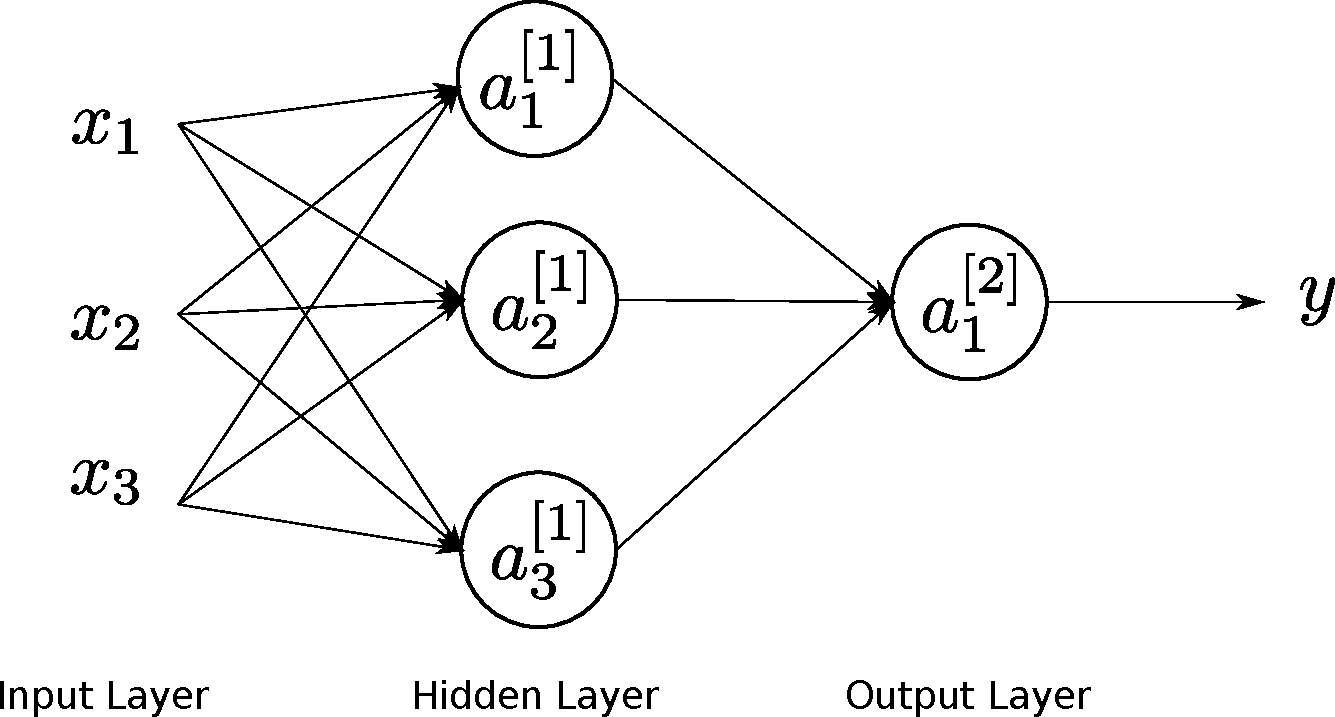
\includegraphics[width=0.6\textwidth]{Chapter4/neuralnet.pdf}
    \caption{Shallow Neural Network Architecture.}
    \label{fig:nn_basic_architecture}
\end{figure}

One last basic definition for NN is the cost function $J(W^{[1]},b^{[1]},...,W^{[L]},b^{[L]})$. The cost function basically measures how good our estimator is to our dataset. The lower the cost function, the less error we obtain when predicting the desired function. Therefore, it represents the target function to be minimized, with respect to all the parameters used in the NN $\{ W^{[1]},b^{[1]},...,W^{[L]},b^{[L]} \}$.

It is possible to employ several different cost functions according to each specific problem. However, we can mention the most common ones, that are the Quadratic Cost, given by Equation \eqref{eq:quadratic_cost}, and the Cross-Entropy Cost, given by Equation \eqref{eq:cross_entropy_cost}.

\begin{equation}
J(W^{[1]},b^{[1]},...,W^{[L]},b^{[L]}) = \frac{1}{m} \sum_{i=1}^{m}{\sum_{j=1}^{n^{[L]}}{ (y_j^{(i)} - a_j^{[L](i)})^2 }}
\label{eq:quadratic_cost}
\end{equation}

\begin{equation}
J(W^{[1]},b^{[1]},...,W^{[L]},b^{[L]}) = \frac{1}{m} \sum_{i=1}^{m}{\sum_{j=1}^{n^{[L]}}{ \left[ y_j^{(i)}\log{a_j^{[L](i)}} - (1-y_j^{(i)}) \log{ (1 - a_j^{[L](i)}) } \right] }}
\label{eq:cross_entropy_cost}
\end{equation}

% describe:
% para cada exemplo de 1 a m, temos um vetor de input x (n[0],1)
% para cada camada de 1 a L, temos:
%			 n[l] hidden units,
%			 uma matriz de parametros W (n[l],n[l-1])
%			 e um vetor de bias b (n[l],1)
% activation functions
% cost function

\subsection{Vectorization}

The previous equations are capable of fully defining update rules for any MLP, however, in order to avoid the naively computation over each training example, and therefore reach more efficient algorithms exploring the use of parallelization in modern GPUs architectures, we must introduce a vectorization notion.

Let's first define the $X$ matrix as the concatenation of each training example $x^{(i)}$ composing its columns, as shown in Equation \eqref{eq:vectorization_concatenation_X}. The matrix $X$ now assumes the dimensions $(n^{[0]},m)$.

\begin{equation}
X = 
\begin{bmatrix}
\vdots & \vdots &  & \vdots \\
x^{(1)} & x^{(2)} & \dots & x^{(m)} \\
\vdots & \vdots &  & \vdots
\end{bmatrix}
\label{eq:vectorization_concatenation_X}
\end{equation}

In this sense, we can analogously define the matrices $A^{[l]}$ and $Z^{[l]}$, as a concatenation of the values for each example $a^{[l](i)}$ and $z^{[l](i)}$, described in Equation \eqref{eq:vectorization_concatenation}. The matrices $A^{[l]}$ and $Z^{[l]}$ now assume the dimensions $(n^{[l]},m)$.

\begin{equation}
A^{[l]} = 
\begin{bmatrix}
\vdots & \vdots &  & \vdots \\
a^{[l](1)} & a^{[l](2)} & \dots & a^{[l](m)} \\
\vdots & \vdots &  & \vdots \\
\end{bmatrix}
\text{ }
Z^{[l]} = 
\begin{bmatrix}
\vdots & \vdots &  & \vdots \\
z^{[l](1)} & z^{[l](2)} & \dots & z^{[l](m)} \\
\vdots & \vdots &  & \vdots \\
\end{bmatrix}
\label{eq:vectorization_concatenation}
\end{equation}

The update equations for each layer, in the vectorized representation, is therefore modified and given by the Equations \eqref{eq:linear_update_nn_vectorized} and \eqref{eq:non_linear_update_nn_vectorized}.

\begin{align}
Z^{[l]} = W^{[l]}A^{[l-1]} + b^{[l]}
\label{eq:linear_update_nn_vectorized}
\\
A^{[l](i)} = g^{[l]}(Z^{[l]})
\label{eq:non_linear_update_nn_vectorized}
\end{align}

\subsection{Forward Propagation}

Given all the definitions of the basic structures of a NN and the main calculations involved, we can derive the algorithm for the forward propagation. The forward Propagation algorithm consists in: given all the dataset composed by the matrix $X$, compute all layers outputs $A^{[l]}$ and $Z^{[l]}$, including the final layer and the final output of the NN, which are $A^{[L]}$ and $Z^{[L]}$.

\begin{algorithm}[H]
    \DontPrintSemicolon
    \SetAlgoLined
    \For{ $l$ = $1$, ..., $L$ }{
        $Z^{[l]} = W^{[l]} A^{[l-1]} + b^{[l]}$\;
        $A^{[l]} = g^{[l]}(Z^{[l]})$\;
        cache $Z^{[l]}$ and $A^{[l]}$\;
    }
    \Return{$A^{[L]}$}
    \caption{Forward Propagation}
    \label{algo:forward_propagation}
\end{algorithm}

\subsection{Backward Propagation}

The ultimate goal in Supervised Learning is minimizing the cost function. For this purpose, one of the most famous optimization techniques used is gradient descent. However, in order to make use of gradient descent, we must compute the derivatives of the cost function with respect to all the parameters $W^{[1]}, b^{[1]}, ..., W^{[L]}, b^{[L]}$. The notation we are going to use for these partial derivatives is given in Equations from \eqref{eq:partial_derivatives_notation_first} to \eqref{eq:partial_derivatives_notation_final}.

\begin{align}
\frac{\partial J(\theta)}{\partial W^{[l]}} = dW^{[l]}
\label{eq:partial_derivatives_notation_first}
\\
\frac{\partial J(\theta)}{\partial b^{[l]}} = db^{[l]} \\
\frac{\partial J(\theta)}{\partial A^{[l]}} = dA^{[l]} \\
\frac{\partial J(\theta)}{\partial Z^{[l]}} = dZ^{[l]}
\label{eq:partial_derivatives_notation_final}
\end{align}

Finding a closed expression for each partial derivative would be a massive analytical work, hence an elegant solution is to employ a iterative algorithm called Backward Propagation, or Backpropagation. The main idea involved in this algorithm is computing each layer output derivative from the next layer output derivative $dA^{[l]}$ and the cached data $A^{[l-1]}$ and $Z^{[l]}$ from the forward propagation algorithm. The Backpropagation algorithm is then given in Algorithm \ref{algo:backward_propagation}.

\begin{algorithm}[H]
    \DontPrintSemicolon
    \SetAlgoLined
    $dA^{L} = \sum_{i=1}^m{\frac{-y^{(i)}}{a^{[L](i)}} + \frac{(1-y^{(i)})}{(1-a^{[L](i)})}}$\;
    \For{ $l$ = $L-1$, ..., $1$ }{
        input $dA^{[l]}$ and cached values $A^{[l-1]}$ and $Z^{[l]}$\;
        $dZ^{[l]} = dA^{[l]} * g'^{[l]}(Z^{[l]})$(element-wise multiplication)\;
        $dW^{[l]} = \frac{1}{m} dZ^{[l]} A^{[l-1]T}$\;
        $db^{[l]} = \frac{1}{m}$ sum over rows of $dZ^{[l]}$\;
        $dA^{[l-1]} = W^{[l]T}dZ^{[l]}$\;
    }
    \Return{($dW^{[1]}, db^{[1]}, ..., dW^{[L]}, db^{[L]}$)}
    \caption{Backward Propagation}
    \label{algo:backward_propagation}
\end{algorithm}

Finally, by making use of the partial derivatives already computed, we can employ the classical Gradient Descent, described in Algorithm \ref{algo:gradient_descent}. Notice that, until convergence, we update all the parameters by the derivatives computed from all the training examples in each step, consisting in the Batch Gradient Descent.

\begin{algorithm}[H]
    \DontPrintSemicolon
    \SetAlgoLined
    Initialize $W^{[1]},b^{[1]},...,W^{[L]},b^{[L]}$ with random values near $0$\;
    \While{ An approximate minimum is not obtained }{
	    Forward Propagation()\;
	    Backward Propagation()\;
   		\For{ $l$ = $1$, ..., $L$ }{
   			$W^{[l]} = W^{[l]} - \alpha dW^{[l]}$\;
   			$b^{[l]} = b^{[l]} - \alpha db^{[l]}$\;
        }
    }
    \Return{($W^{[1]}, b^{[1]}, ..., W^{[L]}, b^{[L]}$)}
    \caption{Gradient Descent}
    \label{algo:gradient_descent}
\end{algorithm}

%\subsection{Optimizations}

\section{Trust Region Policy Optimization}

Given all the RL and NN background necessary, we will introduce two state of the art techniques combining both fields.

The intersection relies on the fact that we need complex non-linear functions to efficiently estimate policies and value-functions. Therefore, the most common used structure for this approximation is MLP. Aiming also to fit stochastic policies distributions in continuous action spaces, we define our policy $\pi_{\theta}(a|s)$ by a normal distribution $\mathcal{N}(\mu,\sigma)$, where the mean $\mu$ and log standard deviation $\sigma$ are outputs of a neural network \cite{TRPO}.

Moreover, in order to work with continuous action spaces, we must employ policy search or actor-critic methods. The classic vanilla policy gradient methods, however, bring some limitations that are handled in the recent techniques. We can cite the main limitation as the vulnerability to the step size in the optimization procedure. This fact brings even bigger impacts due to the non-stationary nature of the input data, which means that a small error in the policy update affects the visitation distribution and consequently the future policy updates.

%The Trust Region Policy Optimization tries to address this limitation. TRPO consists in an on-policy approach that transforms a RL problem into an optimization problem, making policy $\pi$ improves through REINFORCE \cite{REINFORCE} by computing an ascent direction based on data sampled from $\pi$. However, the novel idea introduced by this algorithm is limiting the policy step size to lie within a so called trust region, and thus avoid divergence.

The Trust Region Policy Optimization tries to address this limitation. The novel idea introduced by this algorithm is limiting the policy step size to lie within a so called trust region, and thus avoid divergence. This trust region is computed through the Kullback-Leibler (KL) divergence. The KL divergence is basically a measure of the deviation between two probability distributions, and it is defined as the relative entropy between two continuous random variables $P$, $Q$. Let $p(x)$ and $q(x)$ be the probability density functions of $P$ and $Q$ respectively, the KL divergence, $KL[P,Q]$, is then given by equation \ref{eq:KL_divergence}.

%The trust region is computed through the Kullback-Leibler (KL) divergence. The KL divergence is basically a measure of the deviation between two probability distributions, and it is defined as the relative entropy between two continuous random variables $P$, $Q$. Let $p(x)$ and $q(x)$ be the probability density functions of $P$ and $Q$ respectively, the KL divergence, $KL[P,Q]$, is then given by equation \ref{eq:KL_divergence}.

\begin{equation}
KL[P,Q] = \int_{-\infty}^{\infty}{p(x)\log{\frac{p(x)}{q(x)}}}
\label{eq:KL_divergence}
\end{equation}

TRPO therefore limits the policy gradient step size by applying a KL based constraint \eqref{eq:TRPO_2} to an optimization problem on a slightly modified cost function \eqref{eq:TRPO_1}. The overall algorithm is iteratively, we run episodes and collect data from $\pi_{\theta_{old}}$, compute $\pi_{\theta}$ from the optimization problem and then update $\pi_{\theta_{old}} \leftarrow \pi_{\theta}$. This method is described in Algorithm \ref{algo:TRPO}.

%consists in a constrained optimization problem, given by equations

\begin{align}
\underset{\theta}{\textrm{maximize }} \mathbb{\hat{E}}_{s_t,a_t \sim \pi_{\theta_{old}} } \left[ \frac{\pi_{\theta}(a_t|s_t)}{
\pi_{\theta_{old}}(a_t|s_t)}\hat{A}_t \right]
\label{eq:TRPO_1}
\\
\textrm{subject to } \mathbb{\hat{E}}_{s_t,a_t \sim \pi_{\theta_{old}} } \left[ KL[\pi_{\theta_{old}},\pi_{\theta}(.|s_t)] \right] \leq \delta
\label{eq:TRPO_2}
\end{align}

\begin{algorithm}[H]
    \DontPrintSemicolon
    \SetAlgoLined
    \For{ iteration = $1$, $2$, ... }{
    	Run policy for N trajectories\;
    	Estimate advantage function $\hat{A}(.)$ at all $n$ timesteps\;
    	$\underset{\theta}{\textrm{maximize }} \sum_{n=1}^{N} {\frac{\pi_{\theta}(a_n|s_n)}{\pi_{\theta_{old}}(a_n|s_n)}\hat{A}_n }$\;
    	$\textrm{subject to } \overline{KL}[\pi_{\theta_{old}},\pi_{\theta}(.|s_t)] \leq \delta$\;
    	$\pi_{\theta_{old}} \leftarrow \pi_{\theta}$\;
    }
    \Return{$\pi_{\theta}$}
    \caption{TRPO}
    \label{algo:TRPO}
\end{algorithm}

In this algorithm, we must compute an estimate for the advantage function $\hat{A}_t$. The advantage function is given by $A(s_t,a_t) = Q(s_t,a_t) - V(s_t)$, and it is basically the standard critic function $Q(s_t,a_t)$ subtracted by a unbiased baseline $V(s_t)$ (state-value function) in order to reduce variance. For solving the constrained optimization problem, the conjugate gradient method is generally used.

TRPO presents a great improvement under data efficiency and convergence properties. However, it has a great computational cost, and its implementation through conjugate gradients can be relatively complicated \cite{PPO}.

\section{Proximal Policy Optimization (PPO)}

The Proximal Policy Optimization \cite{PPO} is a recent technique that follows a similar approach used for TRPO, which consists in solving an optimization problem by computing an update at each step that minimizes the cost function while ensuring a relatively small deviation from the previous policy. However, the great breakthroughs introduced are enhancements in the ease of implementation and the ease of hyperparameters tuning, while achieving an even better performance.

The main idea behind TRPO is to use an adaptive KL penalty to control the change of the policy at each iteration. PPO introduces a novel objective function, which intrinsically address this constraint in a first-order optimization.

Let $r_t(\theta)$ be the ratio between the new and old policy, given by the Equation \eqref{eq:def_r_t}, the PPO's objective function is then described by the Equation \eqref{eq:PPO_objective_function}.

\begin{equation}
r_t(\theta) = \frac{\pi_{\theta}(a_t|s_t)}{\pi_{\theta_{old}}(a_t|s_t)}
\label{eq:def_r_t}
\end{equation}

\begin{equation}
L(\theta) = \mathbb{\hat{E}}_t \left[ min(r_t(\theta)\hat{A}_t, clip(r_t(\theta),1-\epsilon,1+\epsilon)\hat{A}_t) \right]
\label{eq:PPO_objective_function}
\end{equation}

In Equation \eqref{eq:PPO_objective_function}, $\theta$ is the policy parameters, $\mathbb{\hat{E}}_t$ is the empirical expectation over all $t$ timesteps, $\hat{A}_t$ is the estimate for the advantage function, as already described, $\epsilon$ is a new hyperparameter, and finally the clip function is explained in Equation \eqref{eq:clip_function}.

\begin{equation}
clip(x,min,max) = \begin{cases}
        min, & \mbox{if } x < min \\
        x, & \mbox{if } min \leq x \leq max \\
        max, & \mbox{if } x > max
        \end{cases}
\label{eq:clip_function}
\end{equation}

PPO does not need complex conjugate gradient techniques, and can be solved with classical stochastic gradient descents. Besides, it has displayed the best performance on continuous control tasks, even compared to TRPO, it also allows parallel implementations and it is very data efficient.

%ease of implementation, sample complexity, and ease of tuning
%compute an update at each step that minimizes the cost function while ensuring the deviation from the previous policy is relatively small.
%TRPO uses an apdtive KL penalty to control the change of the policy at each iteration
%PPO uses a novel objective function which already address this contraint
%present the objective function
%doesnt need complex conjugate gradient techniques, can be solved with the standard stochastic gradient descent
%it has displayed the best performance on continuous control tasks, even compared to TRPO, allows parallel implementations and is very data efficient

